\section{Metodologia}

O aparato experimental foi montado conforme mostra a Fig. \ref{fig: aparato_fh}, seguindo as instruções
do fabricante.\cite{roteiro} 
O gás utilizado foi vapor de mercúrio.
Inicialmente, o potencial de retardo foi mantido constante em $V_r = \qty{2}{\volt}$.
O termostato foi ajustado inicialmente para $\qty{100}{\celsius}$. 
Utilizando o software \textit{Mesure}, foi realizada a medição dos dados seguindo o seguinte protocolo:
\begin{itemize}
\item A chave comutadora era fechada e as medições começavam; 

\item A chave era mantida fechada até o programa avisar que a medição havia sido concluida;

\item O valor de $T$ era alterado e o processo era repetido. 
\end{itemize} 

\begin{figure}[h]
\centering
\caption{Aparato experimental para o experimento de F-H.}
  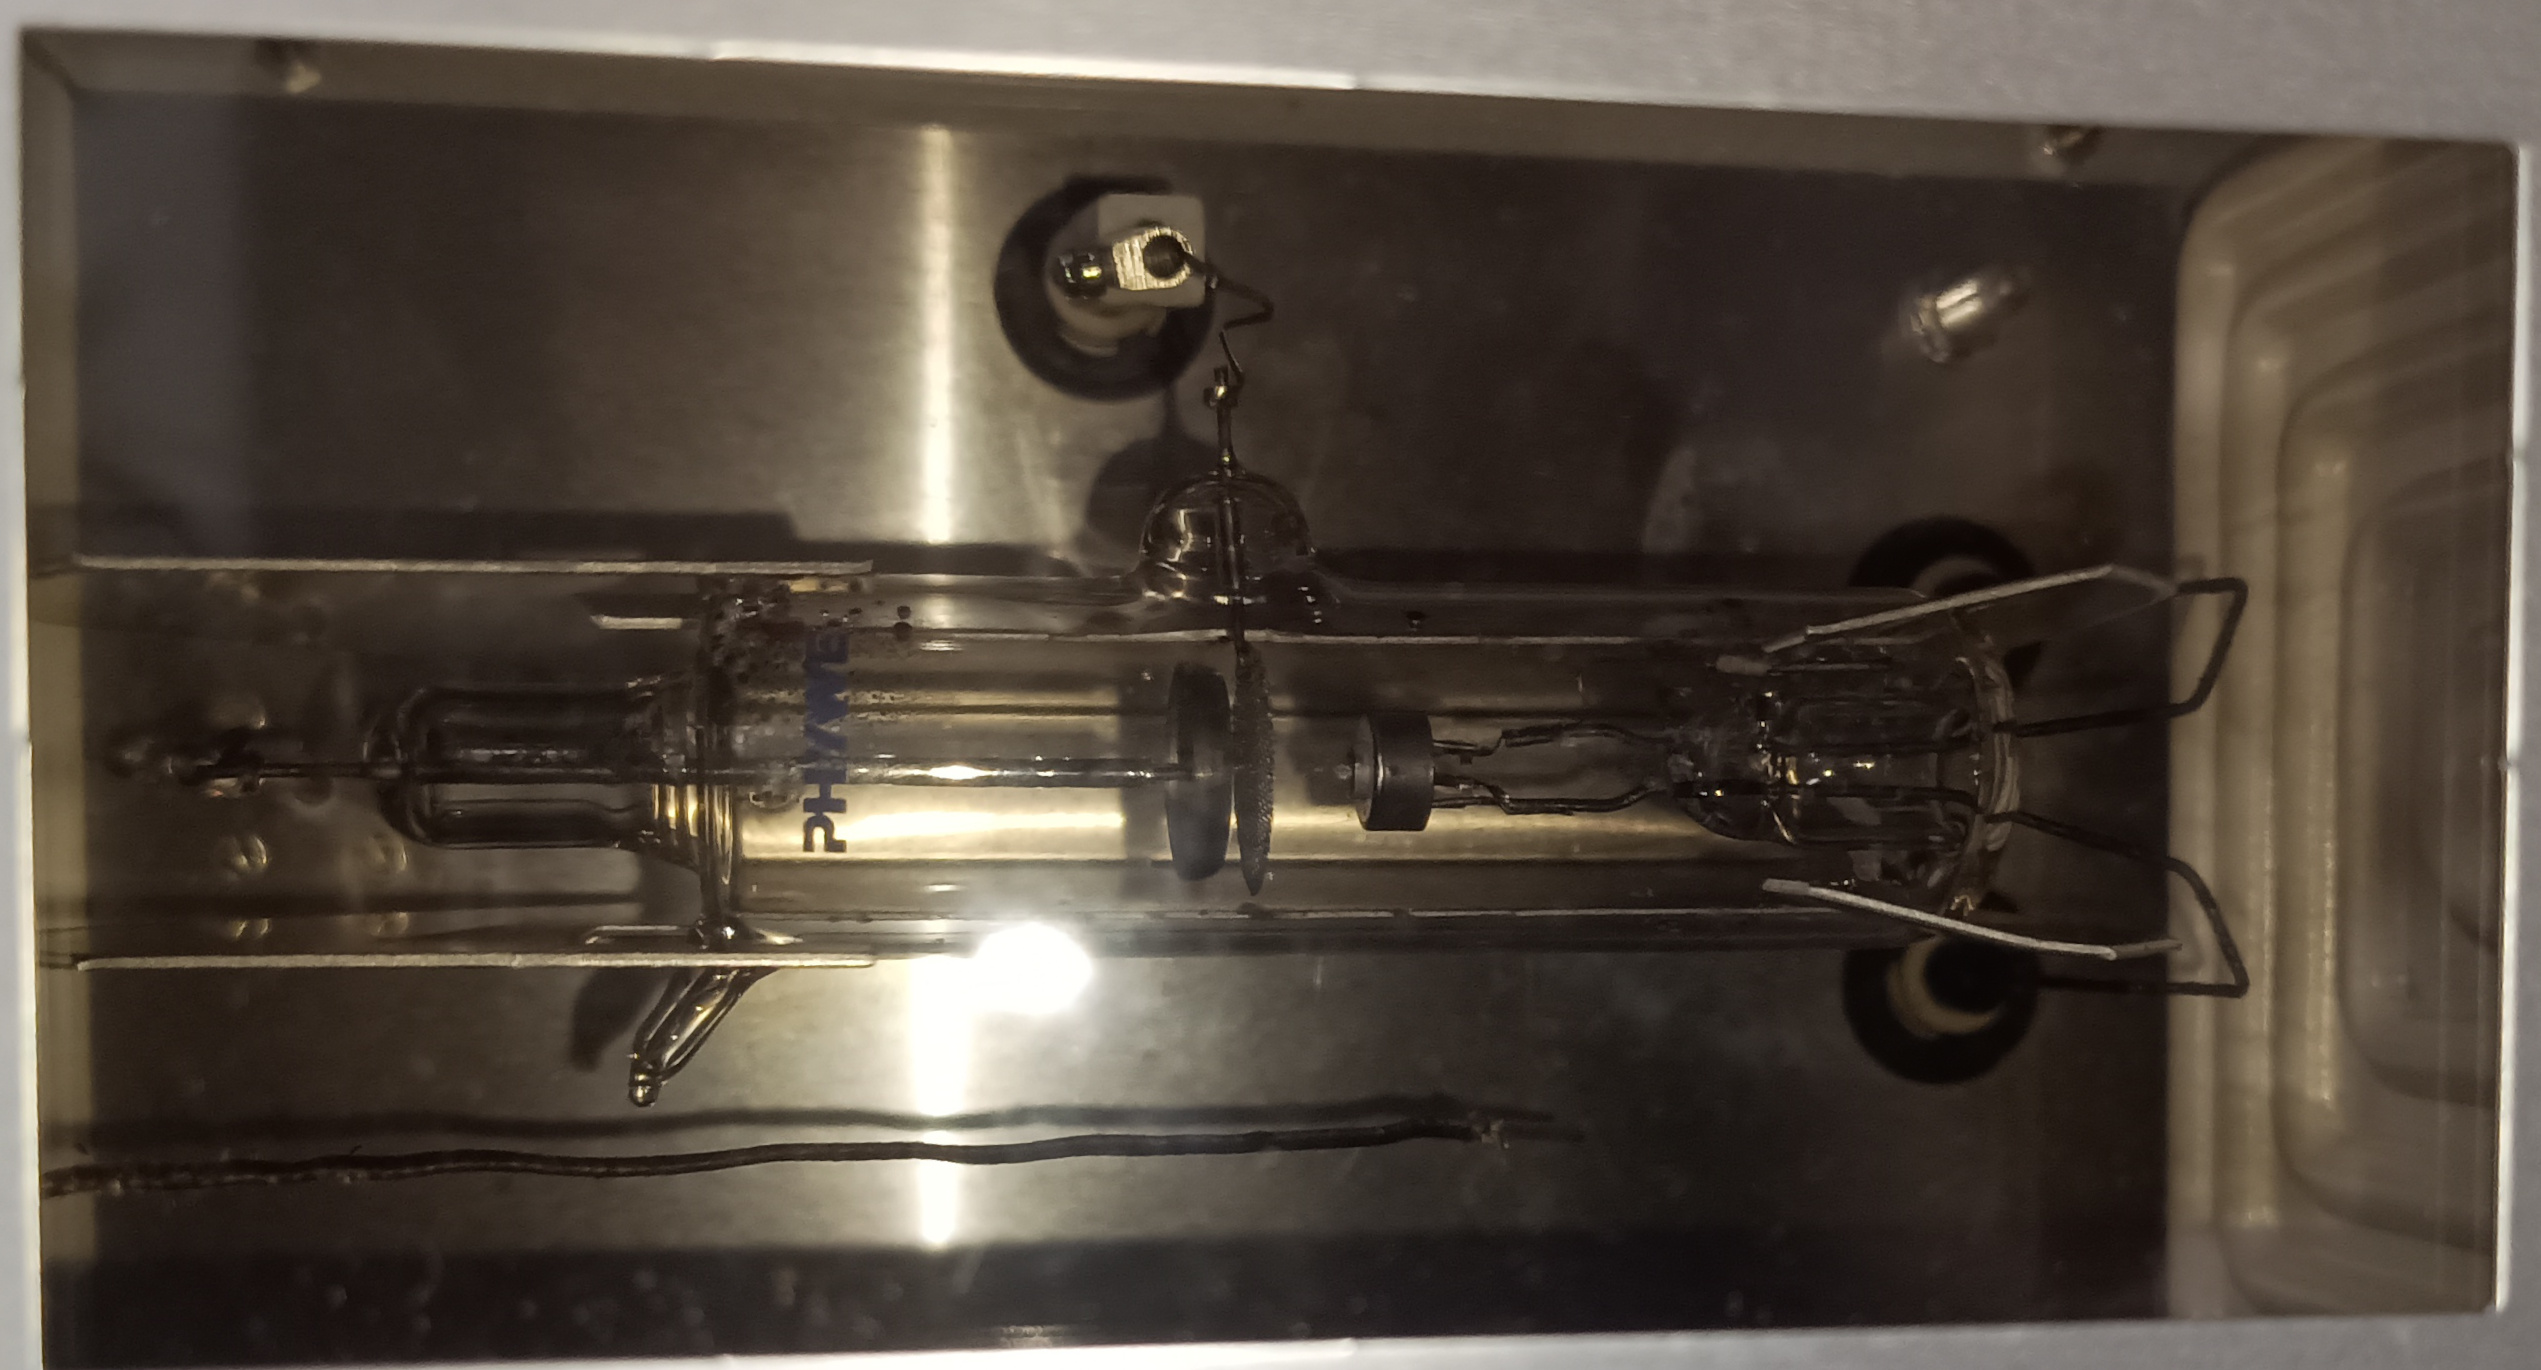
\includegraphics[width=.85\linewidth]{imagens/tubo.jpg}  

  \vspace{4pt} 
  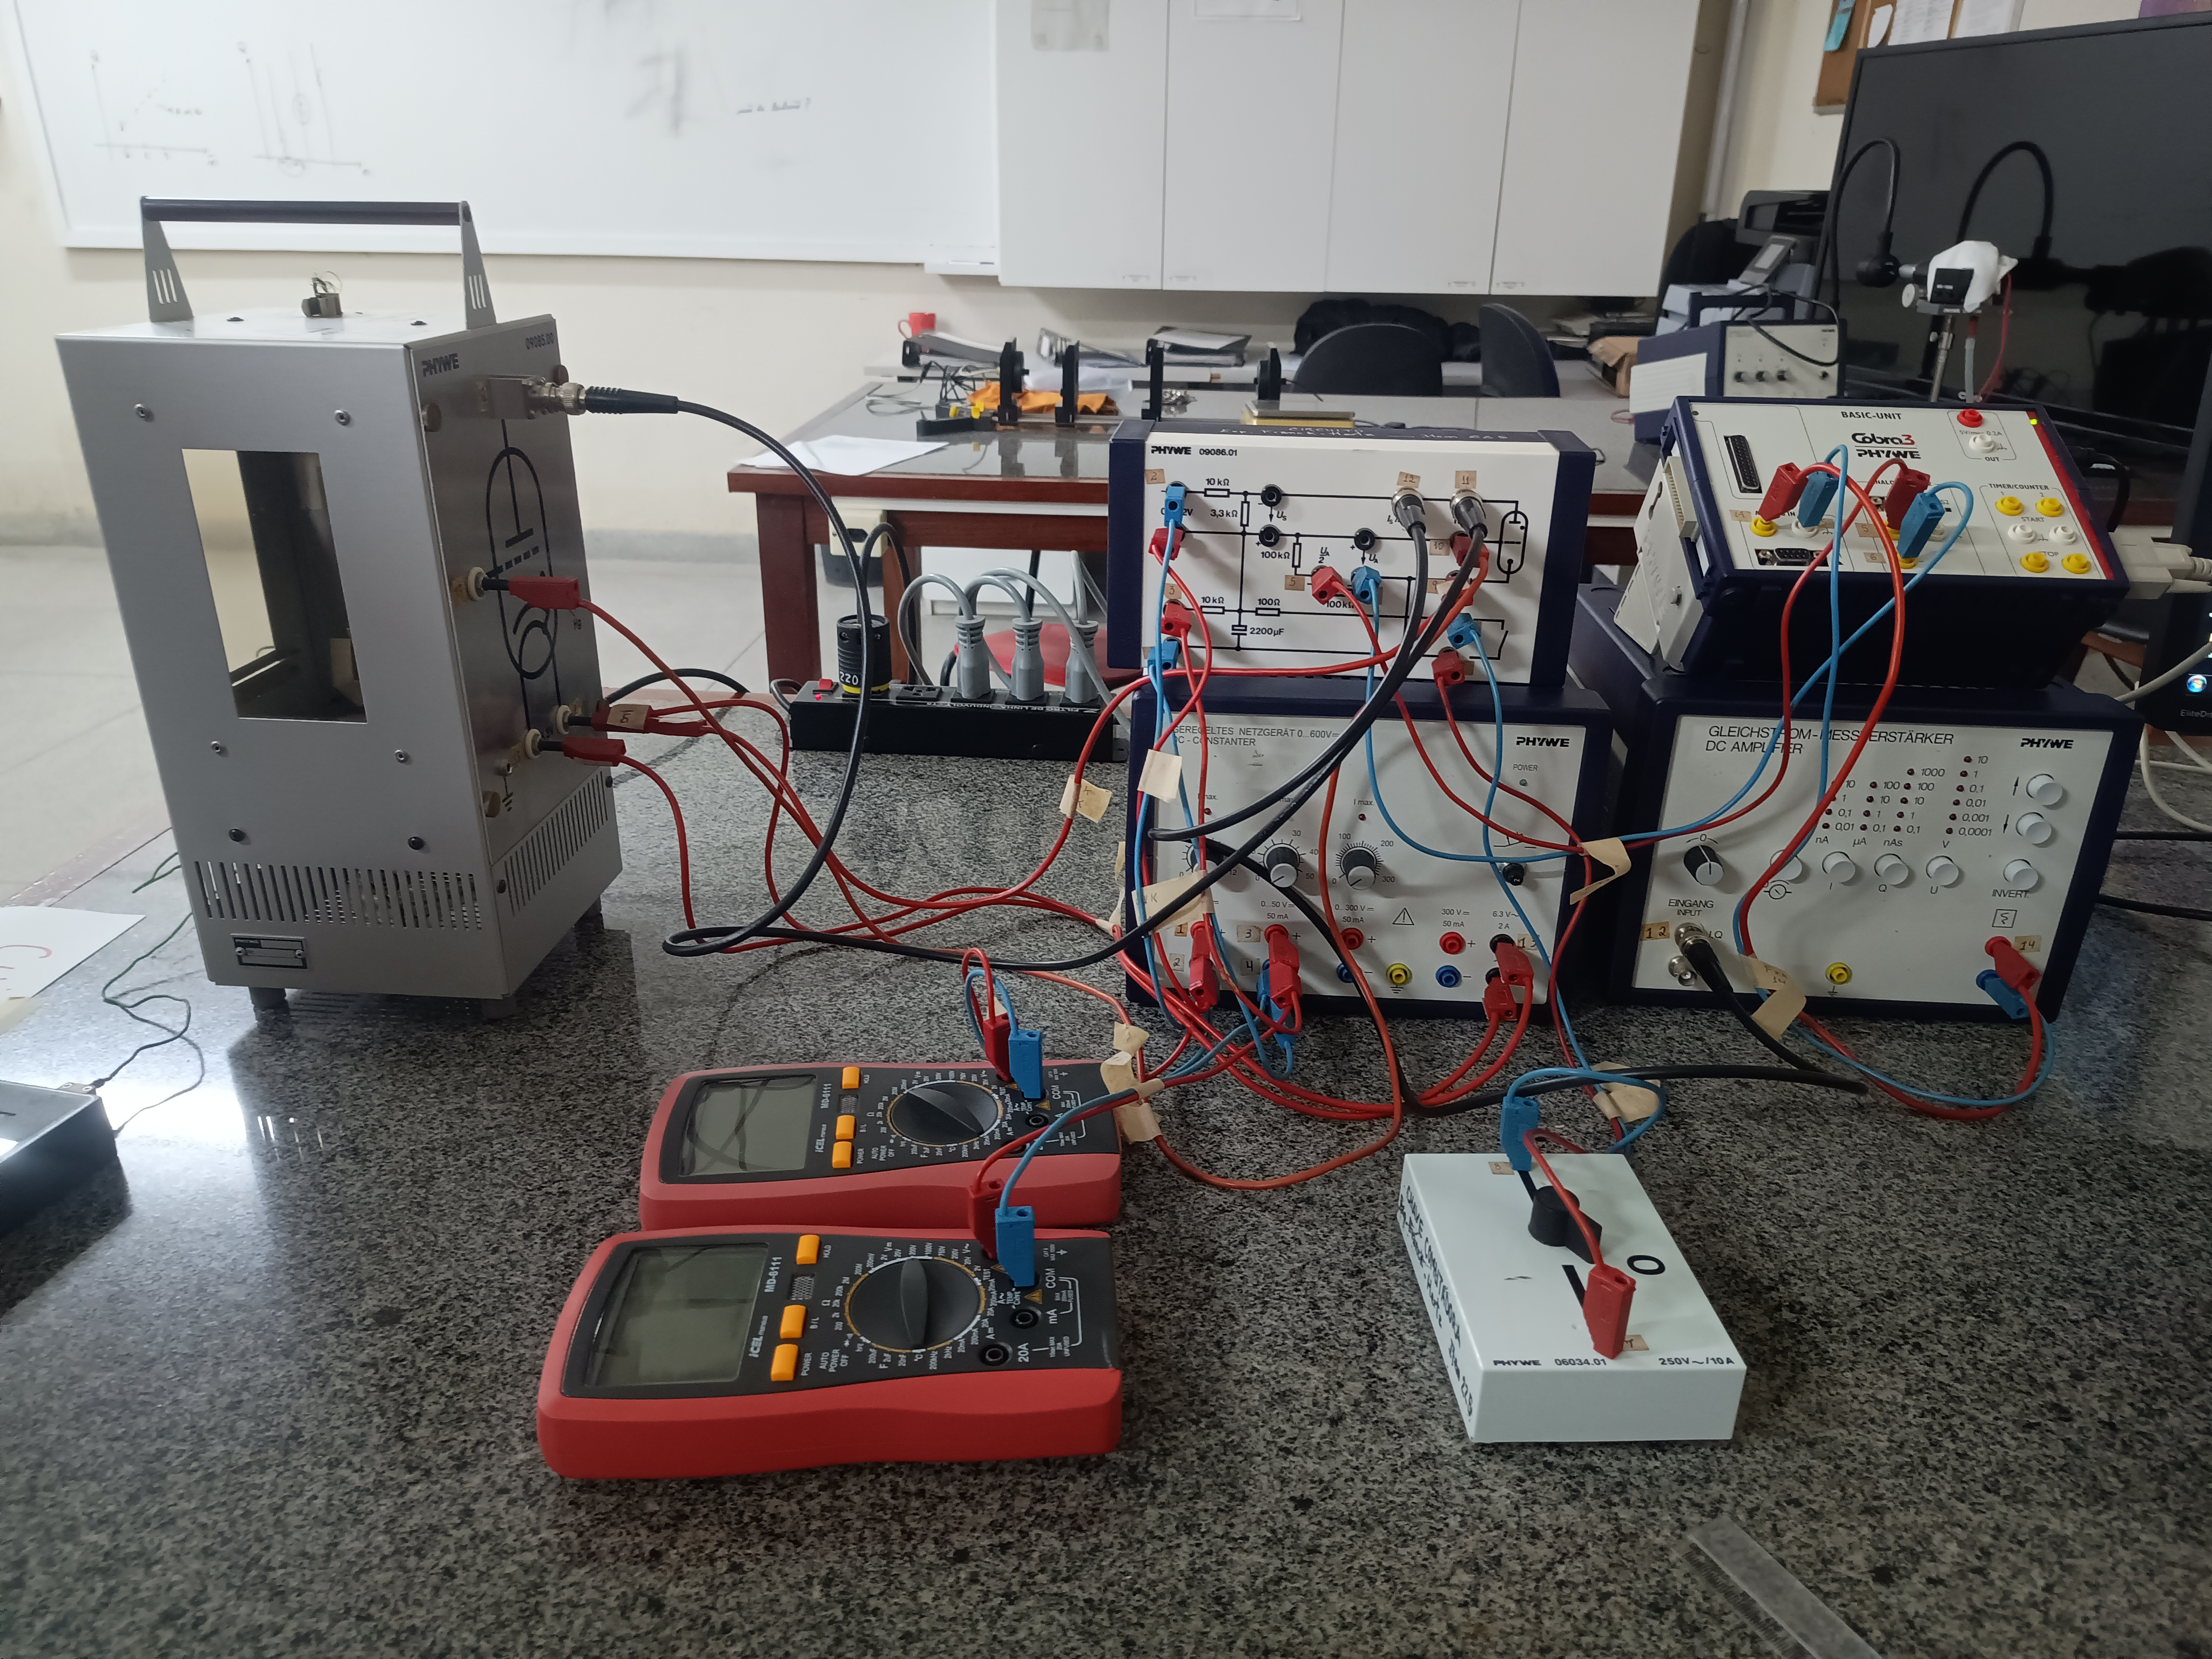
\includegraphics[width=.85\linewidth]{imagens/circuito.jpg}
  {\small \\Fonte: Autor, 2026.}
  \label{fig: aparato_fh}
\end{figure}

Em cada medida, o potencial de excitação $V$ era variado continuamente enquanto o programa registrava os valores de 
$I$ e de $V$.
Foram realizadas medidas até $T=\qty{160}{\celsius}$, com incrementos de $\qty{20}{\celsius}$.

Mantendo agora a temperatura fixa em $\qty{160}{\celsius}$, o processo foi repetido, mas agora variando o valor do potencial
de retardo. Foram realizadas medidas para $V_r = 0,5$, 1, 2, 3, 4, e $\qty{5}{\volt}$.	

% TABELA DE MATERIAIS
\begin{table}
\centering
\caption{Materiais utilizados.}
\begin{tabular}{lc}
\toprule\midrule
Material & Qntd. \\
\midrule
Chave On/off & 1 \\
Termometro digital & 1 \\
Cabo de conexão, 250 mm, vermelho  & 2 \\
Cabo de conexão, 250 mm, azul  & 2 \\
Cabo de conexão, 500 mm, vermelho & 2 \\
Cabo de conexão, 500 mm, azul & 2 \\
Cabo de conexão, 750 mm, vermelho & 3 \\
Cabo de conexão, 750 mm, azul & 1 \\
Cabo de conexão, 2000 mm, vermelho & 2 \\
Cabo de conexão, 2000 mm, azul & 2 \\
Cabo blindado, BNC, l 750 mm & 2 \\
Tubo de Franck-Hertz no prato & 1 \\
Forno de Franck-Hertz & 1 \\
Fonte de alimentação para tubo de F-H & 1 \\
Fonte de alimentação & 1 \\
ermopar NiCr-Ni,500 C máx. & 1 \\ 
Amplificador de medidas DC & 1 \\
Fonte de alimentação, 0...600 V-DC & 1 \\
Cabo de dados PC COBRA RS232, 2m & 1 \\
Capacitor eletrolítico PEK 100mmF/35 V & 2 \\	
Multímetro digital & 2 \\
\midrule\bottomrule
\end{tabular}
\small{\\Fonte: \cite{roteiro}}
\label{tab: materiais}
\end{table}


